\documentclass[12pt, a4paper]{scrbook}

\usepackage[utf8]{inputenc}
\usepackage[a4paper, total={7in, 10in}]{geometry}
\usepackage[T1]{fontenc}
\usepackage[french]{babel}  
%\usepackage{fullpage}

\usepackage[none]{hyphenat}
\usepackage{amsmath}
\usepackage[ruled, linesnumbered, french, onelanguage]{algorithm2e}
\usepackage{babel,csquotes}
\usepackage{listings}
\usepackage{graphicx}  % pour inclure des images
\usepackage[arrowdel]{physics} % pour ajouter le symbole des gradients
\usepackage{subfig}
\usepackage[section]{placeins}
\usepackage[toc,page]{appendix}
\usepackage[backend=biber,
	    style=numeric,
	    citestyle=numeric]{biblatex}

\renewcommand*{\sfdefault}{\familydefault}

\addbibresource{Bibliographie/references.bib}

\graphicspath{ {./images/} }


\title{ Suivi de seiches dans des videos sous-marine}
\subtitle{Projet de programmation 2 }         % Les paramètres du titre : titre, auteur, date
\author{ Vaisse Ariane \and Beldjilali Maxime \and Young Brun Luis-Miguel \and Combe-Ounkham Gabriel \\ \\
		\small{Encadre par} \\ \small{Houda Hammami}}        
\subject{Université de Montpellier\\
		Faculté des Sciences\\
		\emph{L3 informatique}.}
\date{2022-2023}          


\KOMAoptions{open=any}
\begin{document}

\maketitle

\chapter*{Résumé}
Le suivi de seiche dans des vidéos sous-marine prisent en conditions réelles est assez difficile, notamment dû aux mouvements de la camera, au contraste, ou encore à la colorimétrie, qui peut varier d'une vidéo à l'autre.\\
Notre objectif est donc de tester plusieurs approchent afin d'explorer et de proposer des solutions robustes pour le suivi de seiche.\\
\\
Nous avons commencé par apprendre ce qui ce fait de mieux dans le domaine du suivi d'objet, afin d'avoir une idée des différentes techniques ainsi que de leur efficacité.\\
\\
Nous utilisons un filtre à particule comme base de notre algorithme de suivi, il utilisera plusieurs types de descripteurs qui seront comparés entre eux afin de déterminer les plus efficace. Leurs efficacités est mesurés en utilisant la méthode de Pascal VOC, qui consiste à comparer la bounding box de référence avec celle estimée par notre méthode.\\
\\
Le modèle d'intelligence artificielle YOLOv7 est utilisé pour faire la détection initiale de seiches dans les premières frames de la vidéo de manière automatique.\\
\\
Le suivi est amélioré grâce à une étape de prédiction qui permet gérer les cas d'occlusions et de déformation des seiches au cours de la vidéo.

\clearpage

\tableofcontents \clearpage

\listoffigures \clearpage

\listofalgorithms \clearpage


\chapter{Introduction}





\section{Énoncé du problème}
Le suivi d'objet par vision par ordinateur a toujours était, et est encore, un problème suscitant beaucoup d'intérêt et qui fait l'objet de beaucoup de sujet de recherche.\\
En effet, le suivi d'objet apparait dans plein de domaine, comme par exemple:
\begin{itemize}
	\item L'aérospatiale, avec l'arrimage de module a l'ISS, ou encore le suivi de débris spatiaux pour ensuite les faire sortir d'orbites sensibles.
	\item Le militaire, avec le suivi de missile pour interception précise.
	\item L'astrophysique, avec le suivi de corps céleste.
	\item L'étude de population animal, comme l'étude de cycle migratoire ou du comportement de certaines espèces.\\
\end{itemize}

Le projet se place dans le contexte du suivi de seiche en milieu aquatique grâce a des vidéos.\\
Les vidéos sous-marine sont sujettes a beaucoup de difficultés, comme la variation de couleur, de lumière et de contraste d'une image a l'autre, la dégradation de la qualité de la vidéo par des sédiments, les mouvements instables du plongeur, ou encore l'arrière plan qui change.\\
Les solutions implémentées doivent essayer de prendre en compte toutes ces variations ainsi que la forme générale de la seiche au cours de ses mouvements (voir figure \ref{fig:cuttlefish_variation}).\\
Le projet a pour objectif de fournir un outil qui propose des solutions qui répondent a toutes ces contraintes, pour suivre des seiches de façon non intrusive (pas de capteurs sur la seiche suivi), afin de limiter l'interaction humaine avec les seiches.

\begin{figure}[!htbp]
\center
	\subfloat{{\includegraphics[height=3cm]{cuttlefish_variation1.png}}}
	\hspace{0.5cm}
	\subfloat{{\includegraphics[height=3cm]{cuttlefish_variation2.png}}}
	\\
	\subfloat{{\includegraphics[height=3cm]{cuttlefish_variation3.png}}}
	\hspace{0.5cm}
	\subfloat{{\includegraphics[height=3cm]{cuttlefish_variation4.png}}}
\caption{Différentes apparences d'une même seiches dans une vidéo.}
\label{fig:cuttlefish_variation}
\end{figure}
\FloatBarrier
\clearpage





\section{Motivation}
Le suivi d'objet, de manière générale, étant un problème que l'on rencontre dans beaucoup de domaine lié à l'informatique, les précédents exemples n'étant qu'un petit aperçu, il est donc un problème de choix à étudier lors de notre parcours d'études.\\
De plus, il permet d'introduire des concepts et algorithmes fondamentaux, comme le concept de filtrage de signaux, ou d'espace de représentation, ou encore, les algorithmes de filtrage, de descripteurs, ou de mesure de similarité.\\
Ces concepts et algorithmes sont récurrents dans le monde de l'informatique et plus précisément quant il s'agit de faire du traitement du signal ou de la vision par ordinateur.\\
Ce familiariser des à présent avec ces différentes notions pourra grandement nous aider dans la suite de notre parcours.\\




\section{Méthodes}
Il existe beaucoup d'approches possible pour résoudre le problème de suivi d'objet, approches parmi lesquelles ont peut noter:
\begin{itemize}
	\item \textit{Intelligence Artificielle}\newline
	Cette approche est de plus en plus populaire, notamment avec des modèles comme YOLO\cite{redmon_you_2016} ou SSD\cite{liu_ssd_2016}. Ces modèles peuvent directement donner la bounding box de l'objet suivi, sans avoir a faire de traitement sur la sortie du modèle.\\
	Cependant, cette approche est peu résistante a l'occlusion de l'objet suivi.\\
	
	\item \textit{Capteurs}\newline
	Cette approche utilise, par exemple, des IMUs ou marqueurs infrarouge, qui peuvent donner des informations sur l'accélération linéaire ou angulaire. Ces informations sont ensuite filtrées grâce à des algorithme de filtrage, comme le filtre de Kalman (linéaire ou non), ou encore le filtre à particule.\\
	Cependant, cette approche nécessite de poser des capteurs sur l'objet à suivre.\\
	
	\item \textit{Photogrammétrie}\newline
	Cette approche utilise des descripteurs d'image pour extraire des features importantes et ensuite, matcher ces features avec d'autres images pour pouvoir estimer le déplacement de la camera.\\
	Cependant, cette approche est plus utilise dans le cas ou l'on cherche à savoir ou est-ce que le cameraman ce situe, plutôt qu'un objet qui se trouve dans une image (comme le SLAM).\\
	
	\item \textit{Hybride}\newline
	Cette approche combine différentes parties des méthodes déjà présentées et est celle sur laquelle ce projet est basé.\\
	On utilise l'intelligence artificielle pour détecter un objet d'intérêt à suivre dans une sequence d'image, la partie filtrage de l'approche avec des capteurs pour améliorer nos estimations de l'état de l'objet suivi, et enfin, la photogrammétrie pour récupérer les features intéressantes dans une image et les comparer avec les features d'une image de référence.\\
	Cette approche est cependant assez sensible aux paramètres que nous lui donnons, ainsi qu'a certaines caractéristiques des images données en entrée, comme le contraste, la résolution ou encore la colorimétrie.\\
	Le détaille de cette approche sera donne en partie \hyperlink{chapter.3}{3}.\\
\end{itemize}





\section{Cahier des charges}

\subsection{Besoins fonctionnels}
Les besoins peuvent être séparés en 5 catégories:
\begin{enumerate}
	\item Le besoin d'une intelligence artificielle pour effectuer la détection initiale.
	\item Le besoin de descripteurs pour récupérer un vecteur qui décrit une image donnée.
	\item Le besoin de mesures de similarité pour comparer un vecteur caractéristique d'une image avec une descripteur de référence.
	\item Le besoin d'un filtre à particule permettant d'estimer certaines propriétés de la seiche que l'on suit.
	\item Le besoin d'un programme principal permettant d'agencer chacune des parties ensemble.\\
\end{enumerate}

Les différents descripteurs et mesures de similarité devront pouvoir être utilise par le filtre à particule afin de mettre à jour l'état de chacune des particules. Par extension, le filtre à particule devra être modulable, afin de fonctionner avec ces différents descripteurs et mesures de similarité, ainsi que de répondre aux demandent du programme principale.\\
Le programme principale ce charge de l'initialisation des différents modules ainsi que de l'affichage de données clefs (visualisation de  résultats).\\

\subsection{Besoins non-fonctionnels}
Les formats vidéos acceptes sont libres.\\
La résolution des vidéos est également libre, mais une préférence sera porte pour la résolution 640x640 (résolution utilise pour entrainer l'intelligence artificielle).\\
Le programme doit pouvoir tourner sur Windows, Linux et OSX.\\
Le programme doit pouvoir sauvegarder le résultat obtenu en une vidéo et également sauvegarder les bounding box dans un fichier texte.\\

\subsection{Contraintes}
Aucun budget n'a été alloue pour le projet, le travail s'effectuera sur nos machines personnelles, ou sur les machines misent à disposition par l'université.\\
Le projet doit être complété en 4 mois, avec une vingtaine de jour supplémentaire pour la rédaction du rapport.\\


\clearpage

\chapter{Technologies}

\section{LabelImg et Roboflow}
LabelImg est un logiciel d'annotation d'image, qui permet entre autre d'annoter une bounding box que l'on dessine sur une image, avec un label que l'on définit, et d'enregistrer le tout sous différent format, comme le Pascal VOC, ou bien le format de YOLO.\\
Ce logiciel a été utilisé pour annoter la vidéo de référence pour que l'on puisse comparer nos résultats avec.\\
\\
Roboflow est un cite en ligne, qui permet de faire de la gestion de base de donnée pour l'entrainement d'intelligence artificielle, ainsi que de l'annotation collaborative.\\
Ce logiciel a été utilisé pour annoter des images de seiche afin de constituer une base de donnée suffisante, pour entrainer l'intelligence artificielle YOLOv7\cite{wang_yolov7_nodate} à détecter des seiches dans une image. L'annotation a été repartie entre les membres du groupe pour accélérer le processus.\\
Une fois l'annotation termine, un dataset a été créé et augmenté grâce à Roboflow, en ajoutant des images déjà annotées auxquelles a été rajouté du bruit, des rotations, ou des changement de contraste et de luminosité. Augmenter ainsi le dataset permet à l'intelligence artificielle d'être plus résistante à des variations de contraste ou de rotation des seiches dans une image.\\




\section{État de l'art de la détection d'objet}




\section{Langage de programmation}
Le langage de programmation choisi est python, un langage très populaire et qui permet de faire du prototypage rapidement. C'est également un des langages les plus utilisé par les chercheurs en intelligence artificielle, notamment avec le framework pytorch.\\
Notre choix a été fait en partie pour cette aspect de prototypage rapide, mais aussi, du fait de notre utilisation du modèle YOLOv7\cite{wang_yolov7_nodate}, qui utilise pytorch.\\
Python possède également une grande quantité de librairie, comme OpenCV, pour le traitement d'image, Numpy, pour les opérations optimisées sur des tenseurs, ou Scipy, pour les calculs scientifiques. Cela nous a permis de nous concentrer sur les algorithmes et de laisser l'affichage d'image et les opérations matricielles à des librairies qui ont été optimisées pour cela.\\
Il a aussi été choisi par ça facilité de prise en main, et parce que tous les membres du groupe ont déjà programmé avec et le maitrise bien.


\clearpage

\chapter{Développements Logiciel : Conception, Modélisation, Implémentation} 

\section{Développements logiciel}
Dans le cadre du projet, plusieurs éléments ont été développé, à noter, une intelligence artificielle pour détecter des seiches dans une image, une base de donnée de seiches pour entraîner l'intelligence artificielle et un algorithme de filtre à particule utilisant des descripteurs et mesures de similarité pour calculer le poids de chaque particule.\\

\subsection{Intelligence Artificielle}
La base de donnée d'image de seiches est composée d'images provenant de vidéos de seiches prises par des plongeurs en mer, et par des particuliers dans des aquariums.\\
Chaque image a été annotée à la main par les membres du groupe en utilisant le logiciel en ligne Roboflow, la base de donnée est constituée d'un total de 5175 images.\\
L'intelligence artificielle utilise le code et les poids pré entrainé de YOLOv7\cite{wang_yolov7_nodate}, qui peuvent être trouvé sur le github officiel de YOLOv7\cite{yolov7_github}.
Cette intelligence artificielle a été entrainée pour 300 cycles de la base de donnée, soit un total de 25 heures sans interruptions.\\
Les performances obtenues sont illustrées dans la figure \ref{fig:ai_results} et des exemples sont donnés en figure \ref{fig:ai_examples}.\\

\begin{figure}[!htbp]
\center
	\subfloat[Precision]{{\includegraphics[scale=0.07]{metricsprecision.png}}}
	\subfloat[Recall]{{\includegraphics[scale=0.07]{metricsrecall.png}}}
	\\
	\subfloat[mAP@.5]{{\includegraphics[scale=0.07]{metricsmAP_0.5.png}}}
	\subfloat[mAP@.5:.95]{{\includegraphics[scale=0.07]{metricsmAP_0.5_0.95.png}}}
\caption{Performances de notre modèle après entrainement.}
\label{fig:ai_results}
\end{figure}
\FloatBarrier

Les différentes définitions peuvent être retrouvées en annexe (\ref{app:mAP}).\\
%Nombre de vrai positif divisé par le nombre de vrai positif plus le nombre de faux positif
%Nombre de vrai positif divisé par le nombre de positif total
\\
Les résultats obtenus sont compilés dans le tableau suivant:\\
\begin{center}
\begin{tabular}{|c|c|c|c|}
	\hline
	Précision & Recall & mAP@.5 & mAP@.5:.95\\
	\hline
	0.953 & 0.959 & 0.971 & 0.607\\
	\hline
\end{tabular}
\end{center}

\begin{figure}[!htbp]
\center
	\subfloat{{\includegraphics[scale=0.3]{cuttlefish_example1.jpg}}}
	\hspace{0.1cm}
	\subfloat{{\includegraphics[scale=0.3]{cuttlefish_example2.jpg}}}
	\\
	\subfloat{{\includegraphics[scale=0.3]{cuttlefish_example3.jpg}}}
	\hspace{0.1cm}
	\subfloat{{\includegraphics[scale=0.3]{cuttlefish_example4.jpg}}}
\caption{Exemples de résultats obtenus par notre modèle.}
\label{fig:ai_examples}
\end{figure}
\FloatBarrier



\subsection{Logiciel de suivi de seiche}
Ce logiciel est composé d'un filtre à particule, de descripteurs, et de mesures de similarité, qui seront développés en partie \hyperlink{chapter.4}{4}.\\
Il prend en entrée une liste de paramètres pour configurer les différentes parties, et une vidéo. Après configuration du filtre à particule, du descripteur et de la mesure de similarité, la première image de la vidéo est donnée à notre intelligence artificielle, pour avoir une estimation de la position et bounding box d'une seiche que l'on souhaite suivre dans la vidéo.\\
Après le traitement de la première image par notre intelligence artificielle, chaque image de la vidéo est donnée au filtre à particule afin qu'il mette à jour toutes ses particules, et estime au mieux la position et la bounding box de la seiche suivie.\\
Une fois que le filtre à particule a fini de traiter une image, celle-ci est affichée avec la position estimée en bleu et la bounding box estimée en vert, et les meilleures particules en rouge (voir figure \ref{fig:soft_result}). Le numéro de l'image traitée est affiché en haut à gauche de la fenêtre.\\

\begin{figure}[!htbp]
\center
	\subfloat{{\includegraphics[scale=0.3]{Cuttlefish_results0013.png}}}
\caption{Exemple d'une image renvoyé par le logiciel.}
\label{fig:soft_result}
\end{figure}
\FloatBarrier

Le logiciel donne également la possibilité de sauvegarder la vidéo résultante, ainsi que les valeurs de la particule estimée à chaque itération du filtre.\\
Sauvegarder cette estimation permet, par la suite, d'effectuer une analyse des performances de nos solutions, en utilisant un script d'évaluation qui calcule l'IoU (voir annexe \ref{app:IoU}) entre une estimation à un instant $t$ et la véritable valeur à ce même instant, comme montré dans la figure \ref{fig:eval_result}.\\

\begin{figure}[!htbp]
\center
	\subfloat{{\includegraphics[scale=0.3]{eval0014.png}}}
\caption{IoU (blanc) entre l'image de référence (vert) et notre résultat (rouge).}
\label{fig:eval_result}
\end{figure}
\FloatBarrier


\clearpage
\section{Modules}
Le diagramme UML de cas d'utilisation (figure \ref{fig:uml_diagram_usecase}) du projet est assez simple, et se résume à une unique relation entre l'utilisateur et le logiciel, celle de lancer le programme avec une vidéo et les paramètres souhaités. Le reste des relations est effectué en interne et aucune interaction externe n'est requise.\\
Le diagramme UML global des classes peut être retrouvé en annexe \ref{app:UMLGlobal}.

\begin{figure}[!htbp]
\center
	\subfloat{{\includegraphics[scale=0.4]{usecase.png}}}
\caption{Diagramme UML de cas d'utilisation.}
\label{fig:uml_diagram_usecase}
\end{figure}
\FloatBarrier


\subsection{Descripteurs}
Le module descripteur est constitué d'une classe parent $Descriptor$ qui possède 5 classes filles, $HOG$, $HOGCASCADE$, $HOGCOLOR$, $LBP$ et $HOGCASCADELBP$. Ces classes sont les différents descripteurs que l'utilisateur peut utiliser dans le filtre à particule.\\
Toutes ces classes possèdent 2 méthodes communes, la méthode $update$ qui permet de mettre à jour certains paramètres du descripteur, et la méthode $compute$ qui permet d'effectuer le calcul du descripteur sur une liste d'images.\\
A noter, que les descripteurs $HOGCASCADE$ et $HOGCOLOR$ sont des variantes du descripteur $HOG$ (HOG et HOG cascade seront détaillés en partie \hyperlink{chapter.4}{4}), et le descripteur $HOGCASCADELBP$ est une combinaison entre un descripteur HOG cascade et LBP.\\
\\
Ce module permet de calculer, pour chaque particule du filtre, un vecteur descripteur qui pourra, par la suite, être comparé avec un descripteur de référence pour estimer la similarité entre la particule et une particule de référence.\\
Le diagramme UML du module est donné en figure \ref{fig:uml_diagram_descriptor}.

\begin{figure}[!htbp]
\center
	\subfloat{{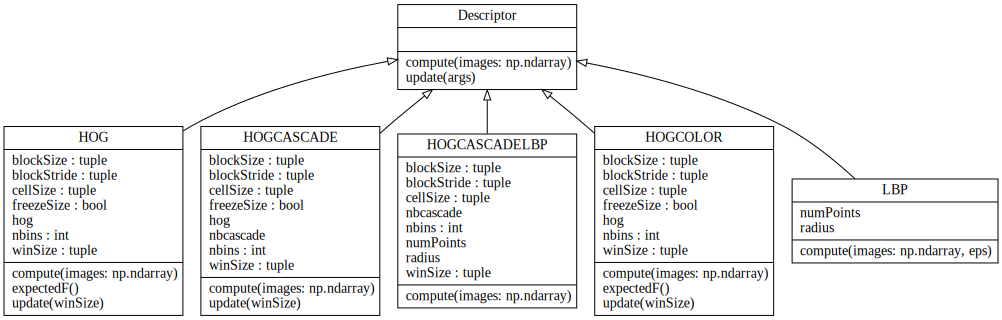
\includegraphics[scale=0.4]{descriptors.png}}}
\caption{Diagramme UML des classes du module descripteur.}
\label{fig:uml_diagram_descriptor}
\end{figure}
\FloatBarrier




\subsection{Mesure de similarité}
Le module mesure de similarité est constitué d'une classe parent $Similarity$ qui possède 4 classes filles, $Bhattacharyya\_sqrt$, $Bhattacharyya\_log$, $Cosine\_Similarity$ et $Kullback\_Leibler\_Divergence$. Ces classes sont les différentes mesures de similarité que l'utilisateur peut utiliser dans le filtre à particule.\\
Toutes ces classes possèdent une méthode commune, la méthode $computeSimilarity$ qui permet de calculer la similarité entre une liste de vecteurs descripteur et un vecteur descripteur de référence.\\
Les mesures de similarité $Bhattacharyya\_sqrt$ et $Cosine\_Similarity$ seront détaillées en partie \hyperlink{chapter.4}{4}.\\
\\
Ce module permet de calculer, pour chaque descripteur de chaque particule du filtre, un coefficient de similarité qui indique quelles particules sont les plus probables de représenter la position de la seiche à un instant $t$.\\
Le diagramme UML du module est donné en figure \ref{fig:uml_diagram_similarity}.

\begin{figure}[!htbp]
\center
	\subfloat{{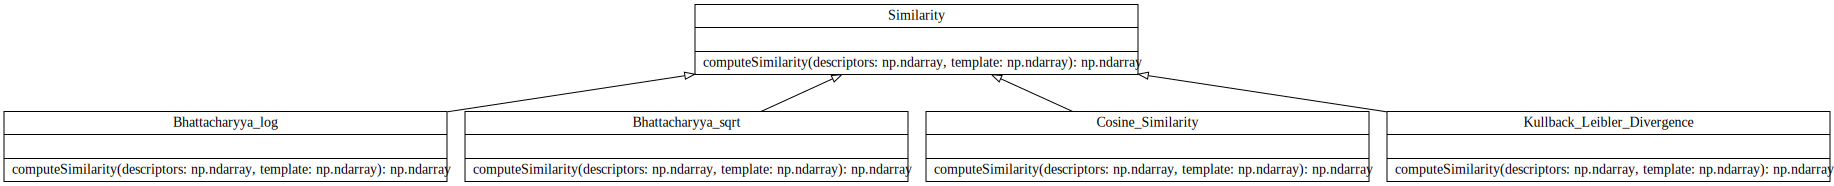
\includegraphics[scale=0.2]{similarity.png}}}
\caption{Diagramme UML des classes du module mesure de similarité.}
\label{fig:uml_diagram_similarity}
\end{figure}
\FloatBarrier




\subsection{Filtre à particule}
Le module filtre à particule est le plus conséquent, car il regroupe plusieurs autres modules, comme les modules descripteur et mesure de similarité. La classe $ParticleFilter$ est la classe principale de ce module et implémente l'algorithme du filtre à particule. Elle fait appel aux classes $Particle$, $Descriptor$, $Slicer$, $Resampling$ et $Similarity$, et les utilisent ensemble pour effectuer le suivi d'une seiche.\\
\\
Ce module est responsable de fournir tous les résultats nécessaires au programme principal, pour qu'il puisse les afficher et/ou les sauvegarder pour être finalement évalués. Ce module est très flexible et permet d'être configuré avec différentes structures de particules, différents descripteurs, différentes mesures de similarité, ou encore différentes méthodes de ré-échantillonnage.\\
Le diagramme UML du module est donné en figure \ref{fig:uml_diagram_particlefilter}.

\begin{figure}[!htbp]
\center
	\subfloat{{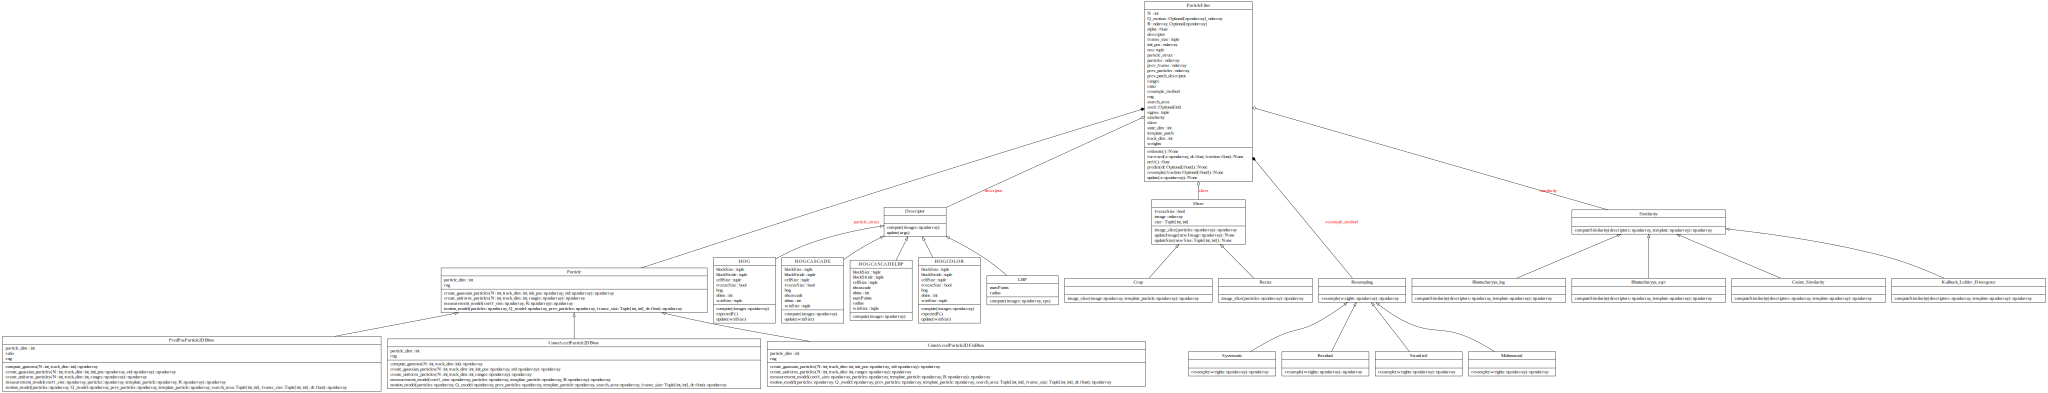
\includegraphics[scale=0.065]{particlefilter.png}}}
\caption{Diagramme UML des classes du module filtre à particule.}
\label{fig:uml_diagram_particlefilter}
\end{figure}
\FloatBarrier





\section{Structures de données}
Les structures de données principales du projet sont les tenseurs en tant que tableaux multidimensionnels, pour ce faire, nous utilisons la librairie Numpy, qui permet de réaliser des opérations sur ces tableaux de façon optimisée.\\
Nous essayons de garder les données un maximum sous ce format, pour éviter les conversions et opérations qui pourraient ralentir le logiciel de suivi. C'est pour cela que la majorité des entrées des programmes réalisés demande des 'ndarray', qui est le type des tableaux Numpy.\\
\\
Les images prises en entrée des programmes sont transformées en tableau Numpy, selon la convention de OpenCV, c'est-à-dire avec les couleurs au format BGR et la hauteur de l'image comme première dimension du tenseur, et la largeur de l'image comme seconde dimension.\\
\\
L'utilisateur du logiciel n'intervient qu'à un seul niveau dans le programme, le reste des entrées du logiciel est géré en interne afin de préserver au mieux l'intégrité des données traitées.\\
L'utilisateur peut uniquement donner des paramètres au logiciel lorsqu'il le lance, ces paramètres sont alors parsés en différent arguments qui sont vérifiés par le programme, puis utilisés pour initialiser les différents modules, afin de commencer le suivi d'une seiche.




\section{Statistiques}
Le projet compte un total de 25 classes réparties dans 10 scripts python (voir figure \ref{fig:uml_diagram_classes}).\\
Les scripts et classes de YOLOv7\cite{wang_yolov7_nodate} utilisés dans le projet ne sont pas comptés.\\
Le projet compte en tout 1587 lignes de code.\\
L'entièreté du projet est en accès libre sur github (\cite{pp2pf}).

\clearpage


\chapter{Algorithmes et Analyse}

\section{Algorithmes}

\subsection{Détection de caractéristiques}

\subsubsection{Descripteurs}

Pour pouvoir appliquer notre mesure de similarité entre deux images et calculer les poids de nos particules, on a besoin de pouvoir extraire de l'information de nos images. Ainsi nous allons utiliser des descripteurs. \\
Un descripteur est un morceau d'information extrait d'une image sous forme de vecteur. Il permettra de reconnaitre un motif ou une structure spécifique au cours de notre vidéo. Pour calculer un descripteur on s'appuie sur l'information bas niveau de nos images (valeur des pixels, contours, gradients, ...).

\subsubsection{Histogramme de gradient orienté}

Nous utiliserons en particulier les histogrammes de gradients orientés (HOG *) qui sont des descripteurs proposés par Navneet DALAL et Bill TRIGGS \cite{dalal_histograms_2005}. Ils correspondent à la distribution de l'orientation des contours locaux d'une image. \\

Les HOG* sont calculés par DALAL et TRIGGS ainsi : \\

Une première étape de pré-traitement de l'image afin de normaliser les couleurs et d'appliquer une correction gamma à celle-ci puis la convertir en niveau de gris. Ici la normalisation du HOG est suffisante et cette étape est donc facultative, on s'est contenté de la conversion en niveau de gris. \\

L'étape suivante est le calcul de la carte des gradients en x et en y qui correspondent respectivement à la variation horizontal et vertical des gradients. On effectue une convolution centrée sur le pixel cible. Parmi les différents filtres possibles, les masques que nous utilisons sont $[-1, 0, 1]$ pour les gradients en x et $[-1, 0, 1]^T$. Ces masques se sont révélés plus performants dans la littérature \cite{dalal_histograms_2005}.\\

À partir de ces deux cartes de gradients on pourrait calculer la carte des modules des gradients. Néanmoins, afin d'augmenter l'efficacité du descripteur, le HOG* n'est pas directement calculer à partir de l'image.\\

En effet l'image est diviser en "cellules", elle-même regroupées en "blocs". On choisit des cellules de 6*6 pixels et des bloc de 3*3 cellules.\\

Pour chaque blocs, on calcule le HOG* de chaque cellule. Le HOG* du bloc correspond à la concaténation du HOG* des cellules le composant. Pour une meilleure invariance face à l'illumination et à l'ombrage on effectue une normalisation du HOG* du bloc (norme euclidiennne). Pour un vecteur x, on a :

\[ \sum_{k=0}^{n} (x_k)^2 \]

Donc le HOG* de l'image est la concaténation de l'ensemble des HOG* de chacun de ses blocs.

\begin{figure}[!htbp]
\center
	\subfloat{{\includegraphics[height=3cm]{Squid_colors_2resized.png}}}
\caption{Bloc d'un HOG*.}
\label{fig:cuttlefish_bloccells}
\end{figure}
\\

Les histogrammes sont construits grâce au mesures des angles des gradients et à leurs intensités. De la même manière qu'avec la taille des blocs et des cellules, on doit choisir la structure de notre histogramme. Étant donnés que nous travaillons sur des angles, nous choisirons un histogramme à neuf classes et nous utiliserons des angles non signés (compris entre $[0; 180^o]$).
Ainsi pour un pixel $p(x,y)$ l'angle est définis par :

\[ angle_p = |\arctan (\grad y, \grad x)*\frac{180}{\pi}| \]

De même que son intensité par :

\[ intensite_p = \sqrt{\grad x^2 + \grad y^2} \]

Pour chaque pixel, on répartit son intensité proportionnellement dans les deux classes les plus proche de l'angle qui lui est associé. 
Par exemple, prenons $\grad x = 10$ et $\grad y = 10$ on obtient un intensité d'environ $14.14$ et un angle de $45^o$. De cette manière la classe centrée en $40$ recevra les trois quarts ($1 - |\frac{5}{20}|$)et la classe centrée en $60$ recevra le quart restant($1 - |\frac{15}{20}|$) de l'intensité.\\

% Note : prendre gradx = grady = sqrt(2) est plus stylé mais je sais pas si c'est sage

Enfin pour affiner notre descripteur nous effectuerons le déplacement du bloc suivant :

\[ \frac{T_cellule * T_bloc}{2} \]

$T_cellule$ est la taille en pixel de la cellule,
$T_bloc$ est la taille en nombre de cellule d'un côté du bloc.
Ainsi on a : $\frac{6*3}{2} = 9$, de plus, un bloc faisant plus de 9 pixels de côté, on a un chevauchement des blocs et donc des pixels pris en compte plusieurs fois. Cela permet au vecteur de mieux caractériser l'image cible.

\begin{figure}[!htbp]
\center
	\subfloat{{\includegraphics[height=3cm]{blocoverlap.png}}}
\caption{Déplacement d'un bloc.}
\label{fig:blocOverlap}
\end{figure}
\\

\subsubsection{HOG* en cascade}

Pour enrichir notre vecteur caractéristique on peut utiliser HOG en cascade qui combines les HOG* de l'image à différentes résolutions. Pour procéder on calcule les HOG* sur une successions de sous-régions inclusives et les ajoutons au HOG* global. De cette manière on ajoute de l'information spatiale à notre descripteur.

\begin{figure}[!htbp]
\center
	\subfloat{{\includegraphics[height=3cm]{Squid_colors_2hogc.png}}}
\caption{HoG en cascade.}
\label{fig:cuttlefish_hog}
\end{figure}
\\

\subsection{Distance de Bhattacharyya}

\subsection{Filtre à particule}

\section{Complexité algorithmique}

\subsection{HOG}

\subsection{Distance de Bhattacharyya}

\subsection{Filtre à particule}

\clearpage

\begin{algorithm}
	\caption{Filtre à particule}\label{alg:particlefilter}
	\KwData{Une vidéo sous-marine de seiche}
	\KwResult{La liste des positions et bounding box de la cible dans la vidéo}
	\ForEach{Images $t$ de la vidéo}{
		\eIf{Première image}{
			Détection de la seiche dans l'image grâce a YOLOv7\\
			Calcul du descripteur de reference : $F_{ref}^{0}$
		}{
			\ForEach{Particules p}{
				Prédiction de la position et de la bounding box de $p$ dans $t$ en fonction de ses états précédents.\\
				Calcul du descripteur du patch correspondant à $p$ : $F_{p}^{t}$\\
				Calcul du poids de $p$ dans $t$ :
					$$w_{p}^{t} = D_{B}(F_{p}^{t},F_{ref}^{t-1})$$
			}
			Ré-échantillonnage des particules pondérées par leurs poids\\
			Estimation de la position et bounding box de la seiche dans $t$ :
				$$X^{t}=\frac{1}{NB_{particule}}*\sum_{p=0}^{NB_{particule}} x_{p}^{t}*w_{p}^{t}$$
		}
		Mise à jour du modèle de référence
	}
\end{algorithm}

\chapter{Analyse des résultats}

\section{Méthodologie}

\section{Analyse et comparaison}

\clearpage

\chapter{Gestion du Projet}

\section{Planification}
Le projet a été divisé entre les 4 membres du groupe pour la partie implémentation des solutions et écriture du rapport, le reste, à savoir, la planification du projet, la répartition des taches et les solutions à implémenter ont été décidé en groupe.\\
La planification c'est faite grâce à un diagramme de Gantt (voir figure \ref{fig:diagram_gantt}) et a été répartie sur les 5 mois accordés, soit du 5 Janvier 2023 au 12 Mai 2023.

\begin{figure}[!htbp]
\begin{ganttchart}[
	hgrid,
	vgrid,
	inline,
	x unit=4mm,
	time slot format=isodate
	]{2023-01-05}{2023-02-19}
	\gantttitlecalendar{week}\\
	\ganttbar{Renseignement}{2023-01-05}{2023-01-15}\\
	\ganttbar{Proposition de solutions}{2023-01-16}{2023-01-29}\\
	\ganttbar{Planification}{2023-01-30}{2023-02-05}\\
	\ganttbar{Rendez-vous}{2023-02-06}{2023-02-12}\\
	\ganttbar{Implémentation}{2023-02-13}{2023-02-19}
	\ganttlink{elem0}{elem1}
	\ganttlink{elem1}{elem2}
	\ganttlink{elem2}{elem3}
	\ganttlink{elem3}{elem4}
\end{ganttchart}
\\
\begin{ganttchart}[
	hgrid,
	vgrid,
	inline,
	x unit=4mm,
	time slot format=isodate
	]{2023-02-20}{2023-04-02}
	\gantttitlecalendar{week=8}\\
	\ganttbar{Implémentation}{2023-02-20}{2023-04-02}
\end{ganttchart}
\\
\begin{ganttchart}[
	hgrid,
	vgrid,
	inline,
	x unit=4mm,
	time slot format=isodate
	]{2023-04-03}{2023-05-12}
	\gantttitlecalendar{week=14}\\
	\ganttbar{Implémentation}{2023-04-03}{2023-04-23}
\end{ganttchart}
\caption{Diagramme de Gantt du projet.}
\label{fig:diagram_gantt}
\end{figure}

\clearpage

\chapter{Bilan et Conclusions}

\clearpage

% Exemple de reference
\cite{xu_human_2010}
\cite{kong_particle_2019}
\cite{qiang_zhu_fast_2006}
\cite{dalal_histograms_2005}
\cite{bhattacharyya_measure_1960}
\cite{rlabbe}


\printbibliography

\begin{appendices}
	%\newgeometry{top=0.7in,bottom=0.7in,left=1in,right=1in}
	
	\chapter*{mAP (mean Average Precision)}\label{appendix:mAP}
\end{appendices}

\clearpage

\end{document}

